\documentclass{article}
\usepackage[margin=1.3in]{geometry}
\usepackage{fancyhdr}
\usepackage{amsmath}
\usepackage{graphics}
\usepackage{graphicx}
\usepackage{amssymb}
\usepackage{setspace}
\usepackage{bm}
\usepackage{ragged2e}
\usepackage{multirow}
\usepackage{fancyhdr}
\usepackage{pgf-umlcd}
\usepackage{tikz}
\usetikzlibrary{automata, positioning, arrows, shapes.geometric}

\tikzset{
	->, % make all edges directed
	>=stealth', % make all arrow heads bold
	node distance = 1.5cm, % min distance between 2 nodes
	every state/.style={thick, fill=gray!10}, % sets the properties for each state node
	initial text=$ $, % sets the taxt that appears on the start arrow
}

\title{\textbf{Cruise Control Software Document}}
\author{
	\textbf{The Spinning Babingos}: \\
	Michael Chunko \\
	Dominick DiMaggio \\
	Ryan Mullens \\
	Alex Heifler \\ \\
	I pledge my honor that I have abided by the Stevens Honor System. \\ \\
	April 4th, 2020 \\ \\
	Version 0.09
}
\date{}

\begin{document}
	\fancypagestyle{plain}{
		\fancyhf{}
		\fancyfoot[c]{\thepage}
	}
	
	\maketitle
	\newpage
	
	\fancypagestyle{plain}{
		\fancyhf{}
		\fancyhead[L]{Michael Chunko, Dominick DiMaggio, Ryan Mullens, Alex Heifler \\ Professor Peyrovian}
		\fancyhead[R]{CS 347 \\ 4 April 2020}
		\renewcommand{\headrulewidth}{.4pt}
		\fancyfoot[c]{\thepage}
	}
	
	\pagestyle{plain}
	
	\tableofcontents
	
	\newpage
	
	\section{Executive Summary}
	\indent\indent The goal of this project is to create an effective cruise control software. The software will be designed so as to run on an embedded system that meets all the stakeholders’ requirements. The software will focus on having an intuitive user experience, so that the user will be able to focus on the road as much as possible. Additionally, the cruise control software will include safety features so as to ensure that the driver is completely safe and and to allow the driver to have a functional cruise control system. 	
	
	\section{Introduction}
	\indent\indent The purpose of our team is to create a cruise control software which runs from an embedded system placed in a contemporary vehicle. There are easily many risks associated with the automation of something so finely managed. Thus the code generated will be rigorously and frequently tested to ensure that there are no unintended or otherwise undesired functionalities in our product. Our cruise control software will be able to assist drivers on the road to drive safely and comfortably. The purpose of our team’s software is to do this well, while ensuring the driver first and foremost remains in control of the vehicle. To that end, we want to stay out of the driver’s way as much as possible, instead working purely to enhance the driving experience and avoiding anything overbearing that would be considered a hindrance. \\
	
	\indent Drivers traveling long distances often become fatigued after staying on the road for an extended period of time. Thanks to our cruise control implementation, the driver will be enabled to make the choice to let their car handle its speed, automatically staying in line with the speed set out by the user. As a result, our software will give users the reprieve they need to remain energized during their potentially long commute. \\
	
	\indent A cruise control system is mission-critical. There is no room for error or unexpected behavior. It is important that nothing is unexpected, lest an accident occur. Our software intends to carry minimal overhead, through use of planned programming practices and optimizations, and leveraging the fact that we are working close to the hardware on this system. During the software development process, our code will be tested thoroughly for fast response times, primarily in response to the driver’s input, but also in interfacing with the sensors across the vehicle that we require for accurate operation. Test cases, use cases, and software specifications will be set concretely by an Agile development process and regular scrums between the team and stakeholders, to ensure that the software will closely match the desired specifications and meet all use cases. \\
	
	\indent We also would like to iterate that responsiveness and effectiveness are not viewed as mutually exclusive. On that thread, we refuse to consider that our software will be working in a pristine environment. While software does not deteriorate in quality, hardware certainly does. Mitigating hardware malfunctions is a major objective throughout our design. Through internal testing and with input from many drivers, we will produce a product that will never leave the driver in a position that will hurt them, regardless of potential hardware failure. More on this will be specified as our process matures.
	
	\newpage
	\section{Requirements}
	\subsection{Functional Requirements}
	\begin{enumerate}
		\item[3.1.1.] The cruise control will activate/deactivate via an input device
		\item[3.1.2.] The cruise control will deactivate by the user pressing the brakes
		\item[3.1.3.] The cruise control will temporarily deactivate while the throttle is pressed, then return to the set speed after the throttle is released
		\item[3.1.4.] The cruise control will have its initial speed set to be the user's current driving speed
		\item[3.1.5.] The cruise control will have its speed adjusted in 1mph increments via an input device
		\item[3.1.6.] The cruise control will log the cruise control speed, if it was activated/deactivated, \textit{why} it was deactivated, and the time all of this occurred
		\item[3.1.7.] The cruise control will use output devices to inform the user of its activation, automatic deactivation, set speed, and if it cannot activate due to too low/high speed
	\end{enumerate}
	
	\subsection{Non--Functional Requirements}
	\begin{enumerate}
		\item[3.2.1.] The cruise control will be highly reliable
		\begin{enumerate}
			\item[3.2.1.a.] It will have a reliability rate equal to or greater than four nines (99.99\%)
		\end{enumerate}
		\item[3.2.2.] The cruise control will react to being activated/deactivated, speed adjustments, and the user pressing the brakes/throttle in 100ms or less
		\begin{enumerate}
			\item[3.2.2.a.] This part of the system is real time and mission critical -- even a small delay could result in accidents occurring 
		\end{enumerate}
		\item[3.2.3.] The cruise control will stay within 0.5mph of the set speed as anything more could result in a negative user experience
		\item[3.2.4.] The cruise control will only work between 25mph (residential road speed limit) and 110mph
		\item[3.2.5.] The cruise control will provide a good user experience
		\begin{enumerate}
			\item[3.2.5.a.] The user should be able to easily use the cruise control system with no prior experience
			\item[3.2.5.b.] The use should be easily made aware of all the info (3.1.7) that they need to know through the output device(s)
		\end{enumerate}
	\end{enumerate}
	
	\subsection{Sensor \& Hardware Requirements}
	\indent\indent As for sensor requirements:
	\begin{enumerate}
		\item[3.3.1.] The cruise control will have a brake sensor (to determine when the user pushes the brakes)
		\item[3.3.2.] The cruise control will have a throttle sensor (to determine when the user pushes the throttle)
		\item[3.3.3.] The cruise control will have access to the speedometer (to properly maintain speed)
		\item[3.3.4.] The cruise control will have a clock (for logging)
	\end{enumerate} \ \\
	\indent And as for hardware requirements:
	\begin{enumerate}
		\item[3.3.5.] The cruise control will have an input device capable of sending data for activation/deactivation
		\item[3.3.6.] The cruise control will have an input device capable of sending data for speed adjustments
		\item[3.3.7.] The cruise control will have output device(s) capable of receiving data for info to display to the user (3.1.7)
		\item[3.3.8.] The cruise control will have a processor capable of doing the needed computing
		\item[3.3.9.] The cruise control will have digital storage with a capacity of 25MB to store the logged information
		\item[3.3.10.] The cruise control will have access to the engine management system to properly control the car's speed
		\item[3.3.11.] The cruise control will have access to both the car's battery and alternator to use as a power source
	\end{enumerate}
	
	\subsection{Security Requirements}
	\indent\indent In order to ensure that the cruise control system is secure it will have the following requirements:
	\begin{enumerate}
		\item[3.4.1.] The cruise control log file will only be able to be accessed through a hardware port
		\item[3.4.2.] Read access to the cruise control log file will be password protected
		\item[3.4.3.] Only the cruise control system will have write access to its log file
		\item[3.4.4.] The cruise control log file will keep track of all read requests and whether or not access was granted
		\item[3.4.5.] The cruise control shall have no connection to the internet, Bluetooth, or other similar networks
		\item[3.4.6.] The only source of input/output for the cruise control will be through the sensor and hardware requirements enumerated in Section 3.3 (3.3.1-3.3.11)
	\end{enumerate}
	
	\newpage
	\section{Requirements Analysis Modeling}
	\indent\indent For brevity's sake, ``CC" is occasionally used in place of ``cruise control" throughout this section.
	
	\subsection{UML Use Cases \& Diagrams}
	\indent\indent Note that the use cases here refer to input/output devices such as a display screen or a button. The cruise control software is only required to provide proper input and output, devices are not specified. We use these device names here for ease of reading.
	\addcontentsline{toc}{subsubsection}{4.1.1\quad Use Case 1}
	\subsubsection*{4.1.1\quad Use Case 1: User's first time using the cruise control system:}
	\begin{itemize}
		\item While driving out of their neighborhood at 20mph, the user attempts to activate the cruise control out of curiosity
		\begin{itemize}
			\item Because the user is below the minimum speed requirement of 25mph the cruise control does not activate
			\item The light on the knob flashes and a beep plays to inform them of this
		\end{itemize}
		\item The user then tries to set the speed using the knob
		\begin{itemize}
			\item The speed on the display screen will not go below 25mph and will not allow the user to enable cruise control until they reach this speed
			\item The user is made aware of the minimum speed requirement
		\end{itemize}
		\item The user makes it to the highway and activates cruise control by pressing the button
		\item It works as the user expects (maintains the set speed)
		\item The user later spots something in the road and suddenly presses the brakes
		\item The cruise control automatically disables
		\begin{itemize}
			\item This is to ensure that the user is always in full control of the vehicle
			\item The user is again informed of this via a beep and a flashing light
		\end{itemize}
	\end{itemize}
	
	\begin{figure}[!htb]
		\centering
		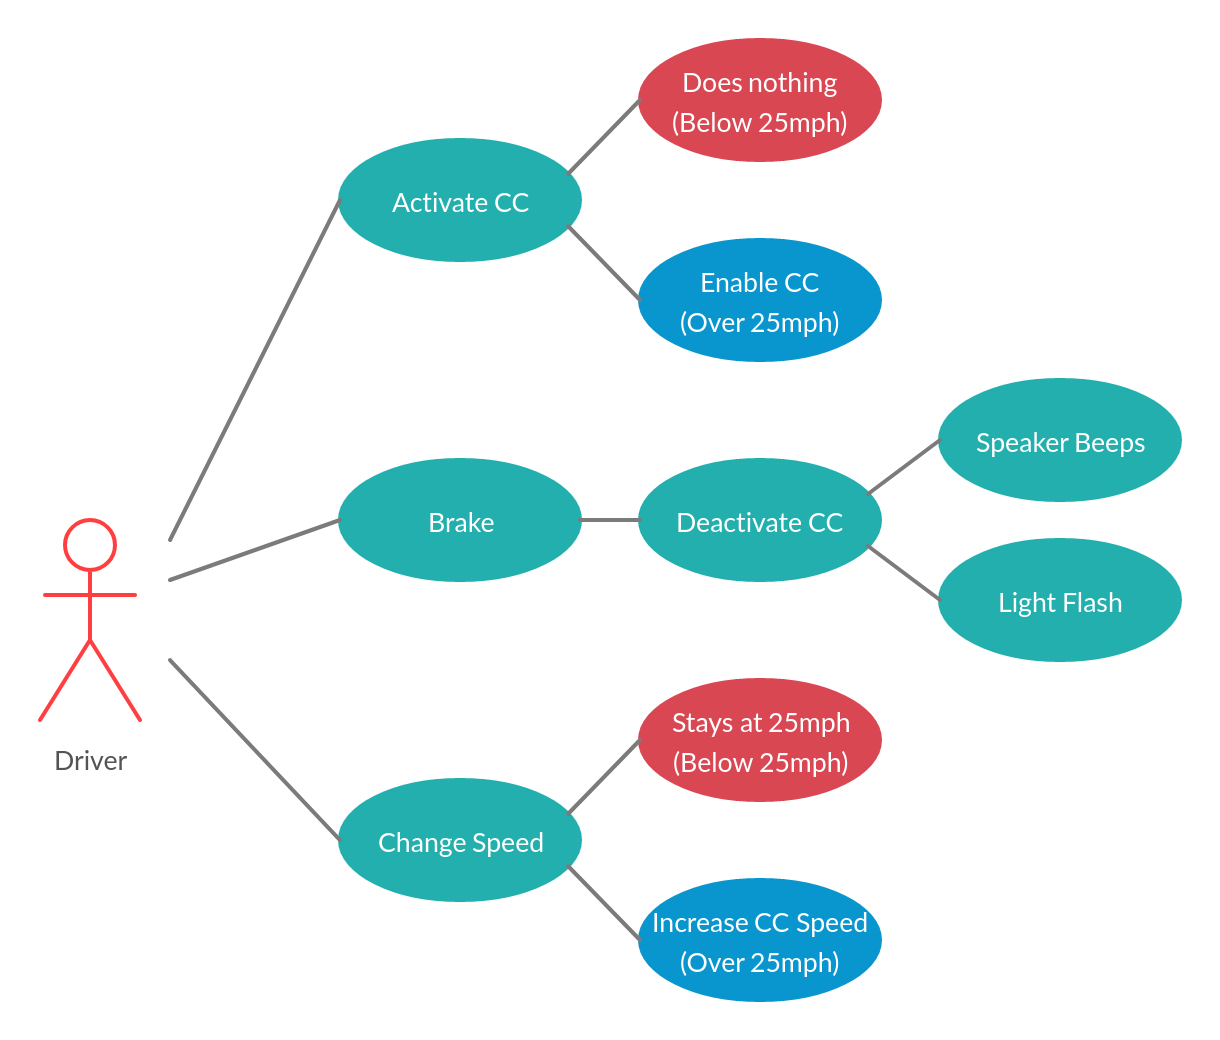
\includegraphics[scale=0.184]{UseCase1}
	\end{figure}
	\newpage
	\addcontentsline{toc}{subsubsection}{4.1.2\quad Use Case 2}
	\subsubsection*{4.1.2\quad Use Case 2: User is cruising down the highway}
	\begin{itemize}
		\item While using cruise control on the highway, the user presses the throttle to overtake another car
		\begin{itemize}
			\item The cruise control temporarily deactivates to allow the user full control over the vehicle
			\item After the throttle is released cruise control is automatically re--activated at the same speed that was previously set
		\end{itemize}
		\item The user gets on to a stretch of highway with a higher speed limit
		\item The user adjusts the set cruise control speed to match this new limit
		\begin{itemize}
			\item The displayed speed changes to reflect the user's new settings and is confirmed by a button press
			\item The cruise control system adjusts the car's speed to this new speed at a comfortable rate
		\end{itemize}
	\end{itemize}
	
	\begin{figure}[!htb]
		\centering
		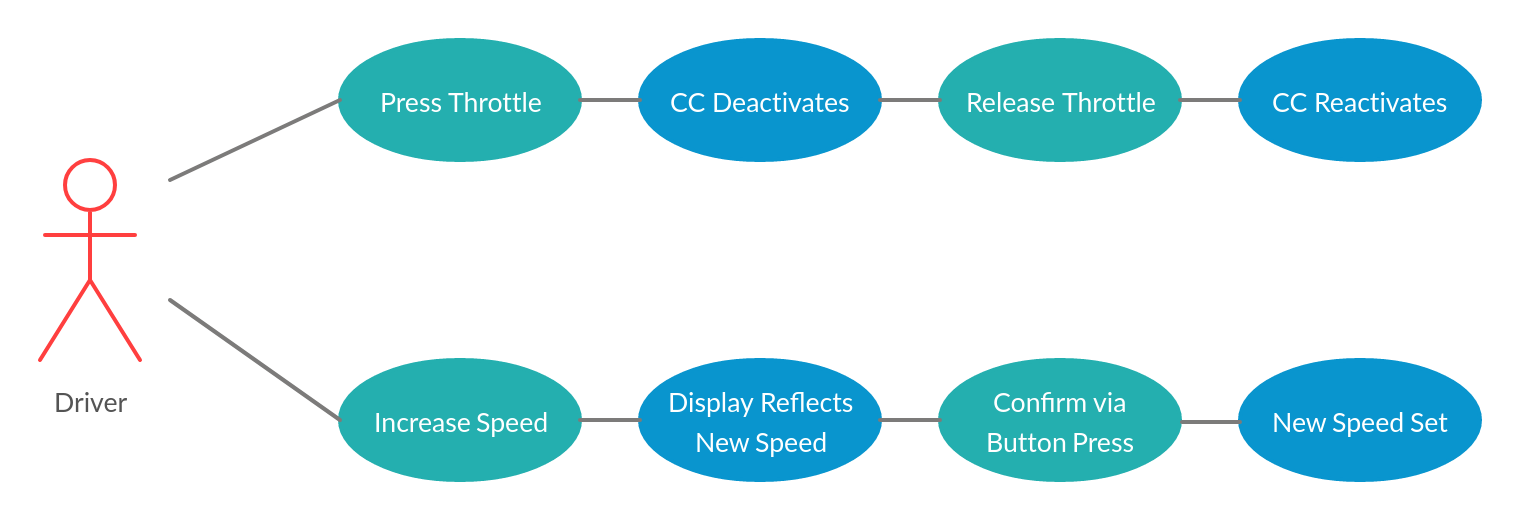
\includegraphics[scale=0.184]{UseCase2}
	\end{figure}
	\newpage
	\addcontentsline{toc}{subsubsection}{4.1.3\quad Use Case 3}
	\subsubsection*{4.1.3\quad Use Case 3: The car goes in for regular maintenance}
	\begin{itemize}
		\item The user brings the car in for regular maintenance
		\item The mechanic accesses the cruise control's log file through the hardware port as specified in Section 3.4 (3.4.1)
		\begin{itemize}
			\item The mechanic is prompted for a password
			\item They enter the manufacturer--provided password and are successfully granted read--only access
		\end{itemize}
		\item From here the mechanic can read the contents of the cruise control log file to ensure that there have been no faults
		\begin{itemize}
			\item The contents of the log file are as specified in Section 3 (3.1.16, 3.4.4)
		\end{itemize}
		\item The mechanic verifies that the cruise control is working as intended and proceeds with the inspection
	\end{itemize}
	
	\begin{figure}[!htb]
		\centering
		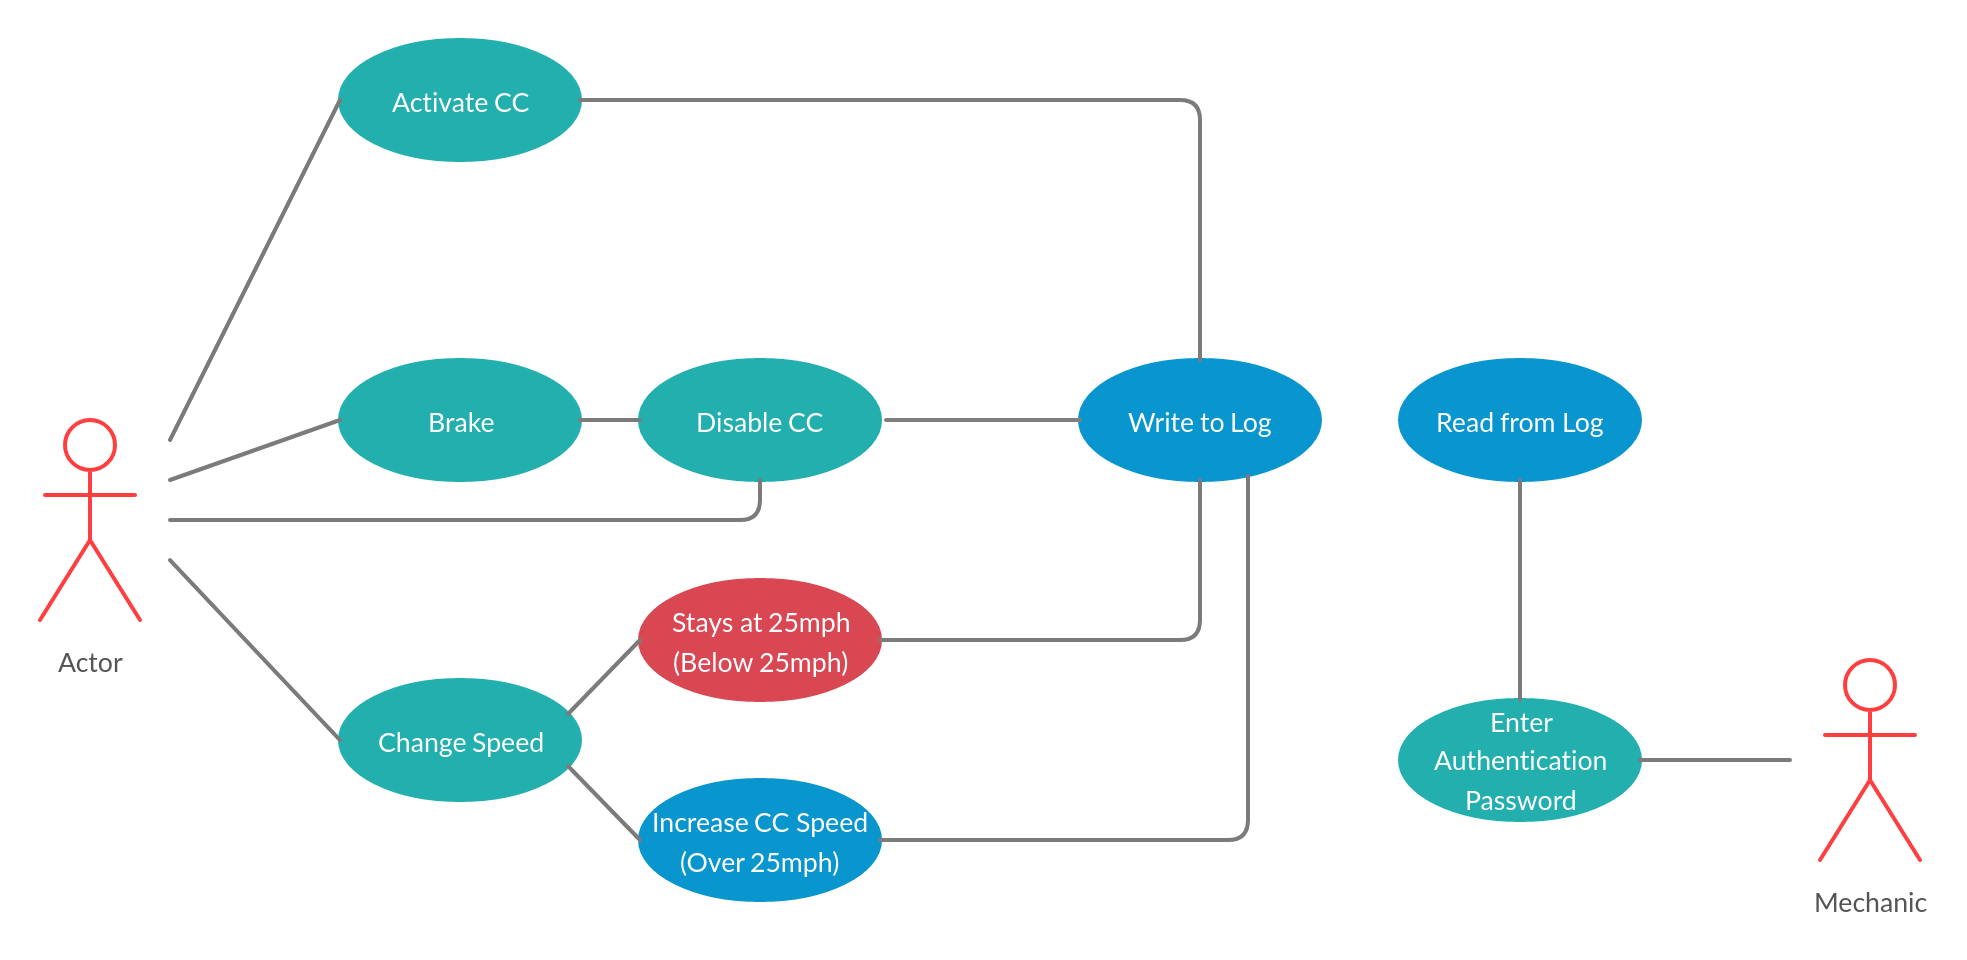
\includegraphics[scale=0.184]{UseCase3}
	\end{figure}
	\newpage
	\addcontentsline{toc}{subsubsection}{4.1.4\quad Use Case 4}
	\subsubsection*{4.1.4\quad Use Case 4: A malicious actor attempts to interfere with the cruise control}
	\begin{itemize}
		\item The user has done something to make the malicious actor attempt to damage the car
		\item The malicious actor starts by trying to damage the cruise control
		\item The malicious actor tries to access the cruise control through the hardware port
		\begin{itemize}
			\item If they do not know the password, the cruise control logs this failed attempt and the malicious actor gets no access
			\item If they somehow do know the password, the cruise control will log the access grant and the malicious actor will get read--only access
		\end{itemize}
		\item If the malicious actor has successfully gotten read--only access, they won't be able to do anything harmful
		\begin{itemize}
			\item Read--only access by definition means that the malicious actor will only be able to read the contents of the log and not modify them in any way
		\end{itemize}
		\item If the malicious actor instead tries getting access to the cruise control through other systems in the car they will fail
		\begin{itemize}
			\item According to Section 3.4 (3.4.5, 3.4.6) the cruise control will not have any unnecessary connections
			\item As the connected systems are also mission critical, their security should provide that there is no way for a malicious actor to gain access to them
		\end{itemize}
	\end{itemize}
	
	\begin{figure}[!htb]
		\centering
		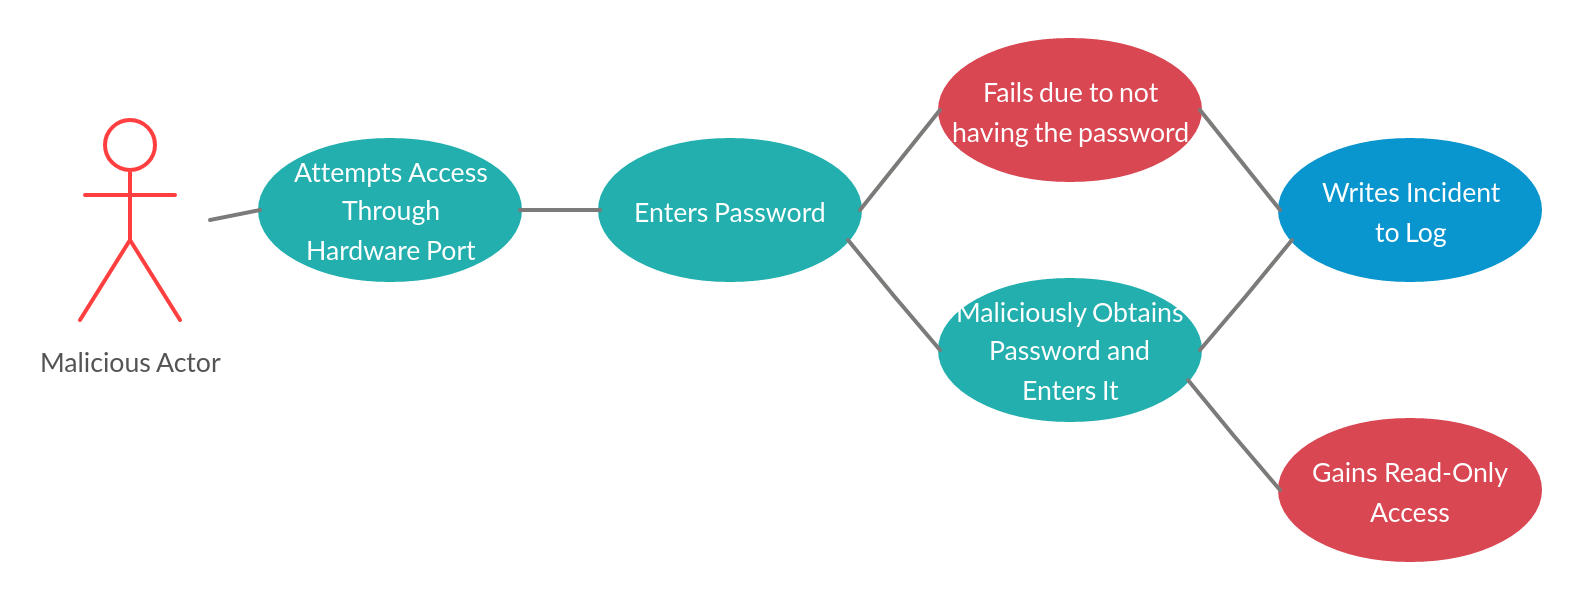
\includegraphics[scale=0.184]{UseCase4}
	\end{figure}
	\newpage
	\subsection{UML Class--Based Modeling}
	\begin{center}
		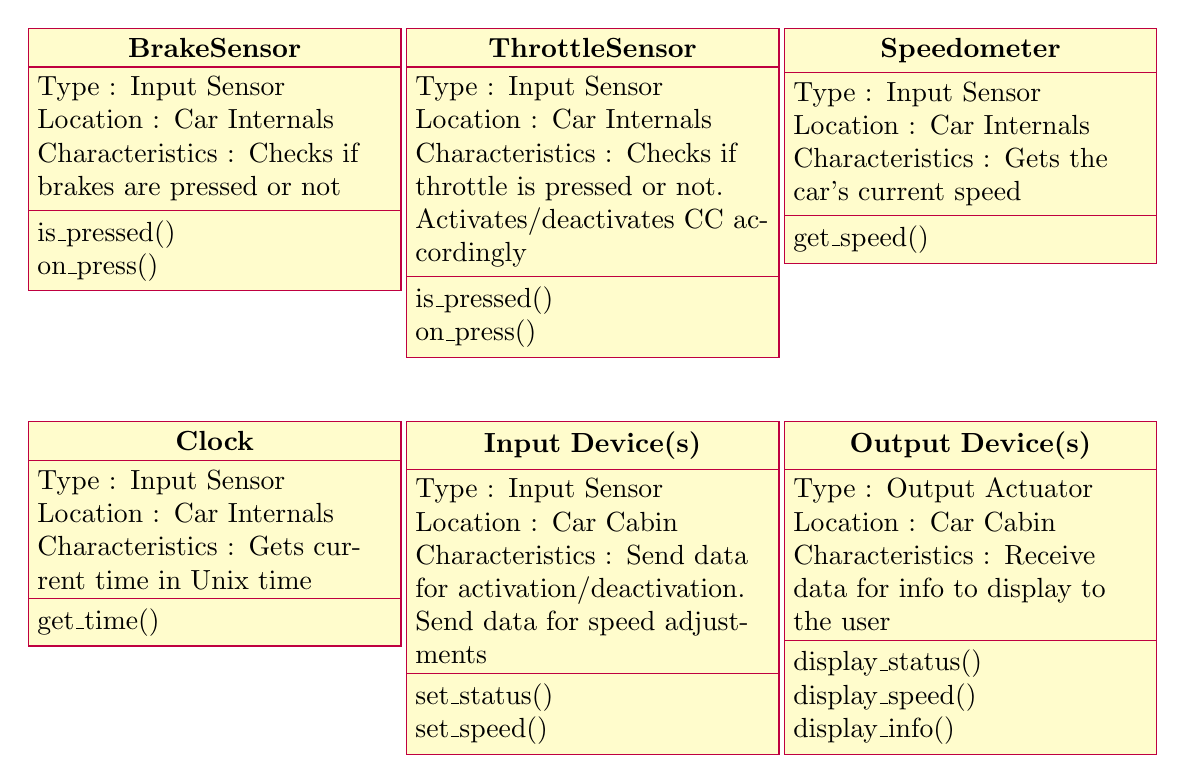
\begin{tikzpicture}
		\begin{class}[text width=4.5cm]{BrakeSensor}{0,0}
		\attribute{Type : Input Sensor}
		\attribute{Location : Car Internals}
		\attribute{Characteristics : Checks if brakes are pressed or not}
		
		\operation{is$\_$pressed()}
		\operation{on$\_$press()}
		\end{class}
		\begin{class}[text width=4.5cm]{ThrottleSensor}{4.8,0}
		\attribute{Type : Input Sensor}
		\attribute{Location : Car Internals}
		\attribute{Characteristics : Checks if throttle is pressed or not. Activates/deactivates CC accordingly}
		
		\operation{is$\_$pressed()}
		\operation{on$\_$press()}
		\end{class}
		\begin{class}[text width=4.5cm]{Speedometer}{9.6,0}
		\attribute{Type : Input Sensor}
		\attribute{Location : Car Internals}
		\attribute{Characteristics : Gets the car's current speed}
		
		\operation{get$\_$speed()}
		\end{class}
		\begin{class}[text width=4.5cm]{Clock}{0,-5}
		\attribute{Type : Input Sensor}
		\attribute{Location : Car Internals}
		\attribute{Characteristics : Gets current time in Unix time}
		
		\operation{get$\_$time()}
		\end{class}
		\begin{class}[text width=4.5cm]{Input Device(s)}{4.8,-5}
		\attribute{Type : Input Sensor}
		\attribute{Location : Car Cabin}
		\attribute{Characteristics : Send data for activation/deactivation. Send data for speed adjustments}
		
		\operation{set$\_$status()}
		\operation{set$\_$speed()}
		\end{class}
		\begin{class}[text width=4.5cm]{Output Device(s)}{9.6,-5}
		\attribute{Type : Output Actuator}
		\attribute{Location : Car Cabin}
		\attribute{Characteristics : Receive data for info to display to the user}
		
		\operation{display$\_$status()}
		\operation{display$\_$speed()}
		\operation{display$\_$info()}
		\end{class}
		\end{tikzpicture}
	\end{center}
	
	\subsection{UML CRC Model Index Cards}
	\begin{center}
		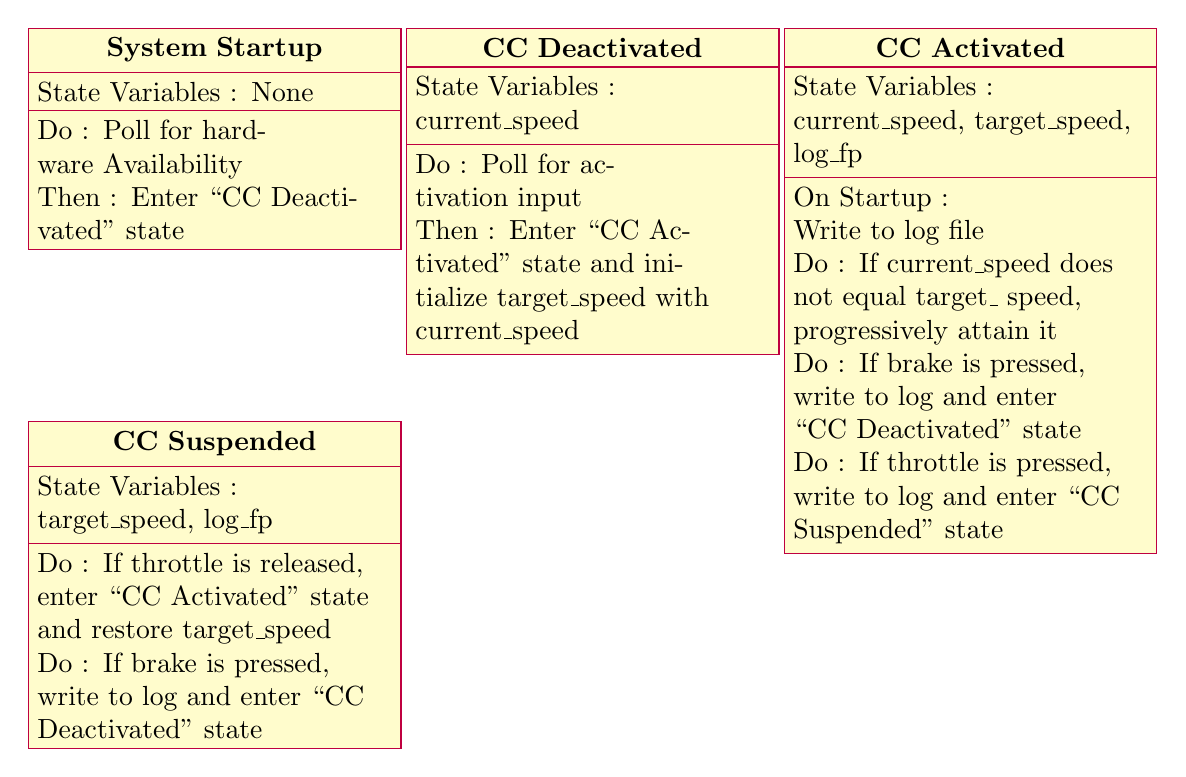
\begin{tikzpicture}
		\begin{class}[text width=4.5cm]{System Startup}{0,0}
		\attribute{State Variables : None}
		
		\operation{Do : Poll for hardware Availability}
		\operation{Then : Enter ``CC Deactivated" state}
		\end{class}
		\begin{class}[text width=4.5cm]{CC Deactivated}{4.8,0}
		\attribute{State Variables : current$\_$speed}
		
		\operation{Do : Poll for activation input}
		\operation{Then : Enter ``CC Activated" state and initialize target$\_$speed with current$\_$speed}
		\end{class}
		\begin{class}[text width=4.5cm]{CC Activated}{9.6,0}
		\attribute{State Variables : current$\_$speed, target$\_$speed, log$\_$fp}
		
		\operation{On Startup : Write to log file}
		\operation{Do : If current$\_$speed does not equal target$\_$ speed, progressively attain it}
		\operation{Do : If brake is pressed, write to log and enter ``CC Deactivated" state}
		\operation{Do : If throttle is pressed, write to log and enter ``CC Suspended" state}
		\end{class}
		
		\begin{class}[text width=4.5cm]{CC Suspended}{0,-5}
		\attribute{State Variables : target$\_$speed, log$\_$fp}
		
		\operation{Do : If throttle is released, enter ``CC Activated" state and restore target$\_$speed}
		\operation{Do : If brake is pressed, write to log and enter ``CC Deactivated" state}
		\end{class}
		\end{tikzpicture}
	\end{center}
	
	\newpage
	\subsection{UML Activity Diagram}
	\begin{figure}[!htb]
		\centering
		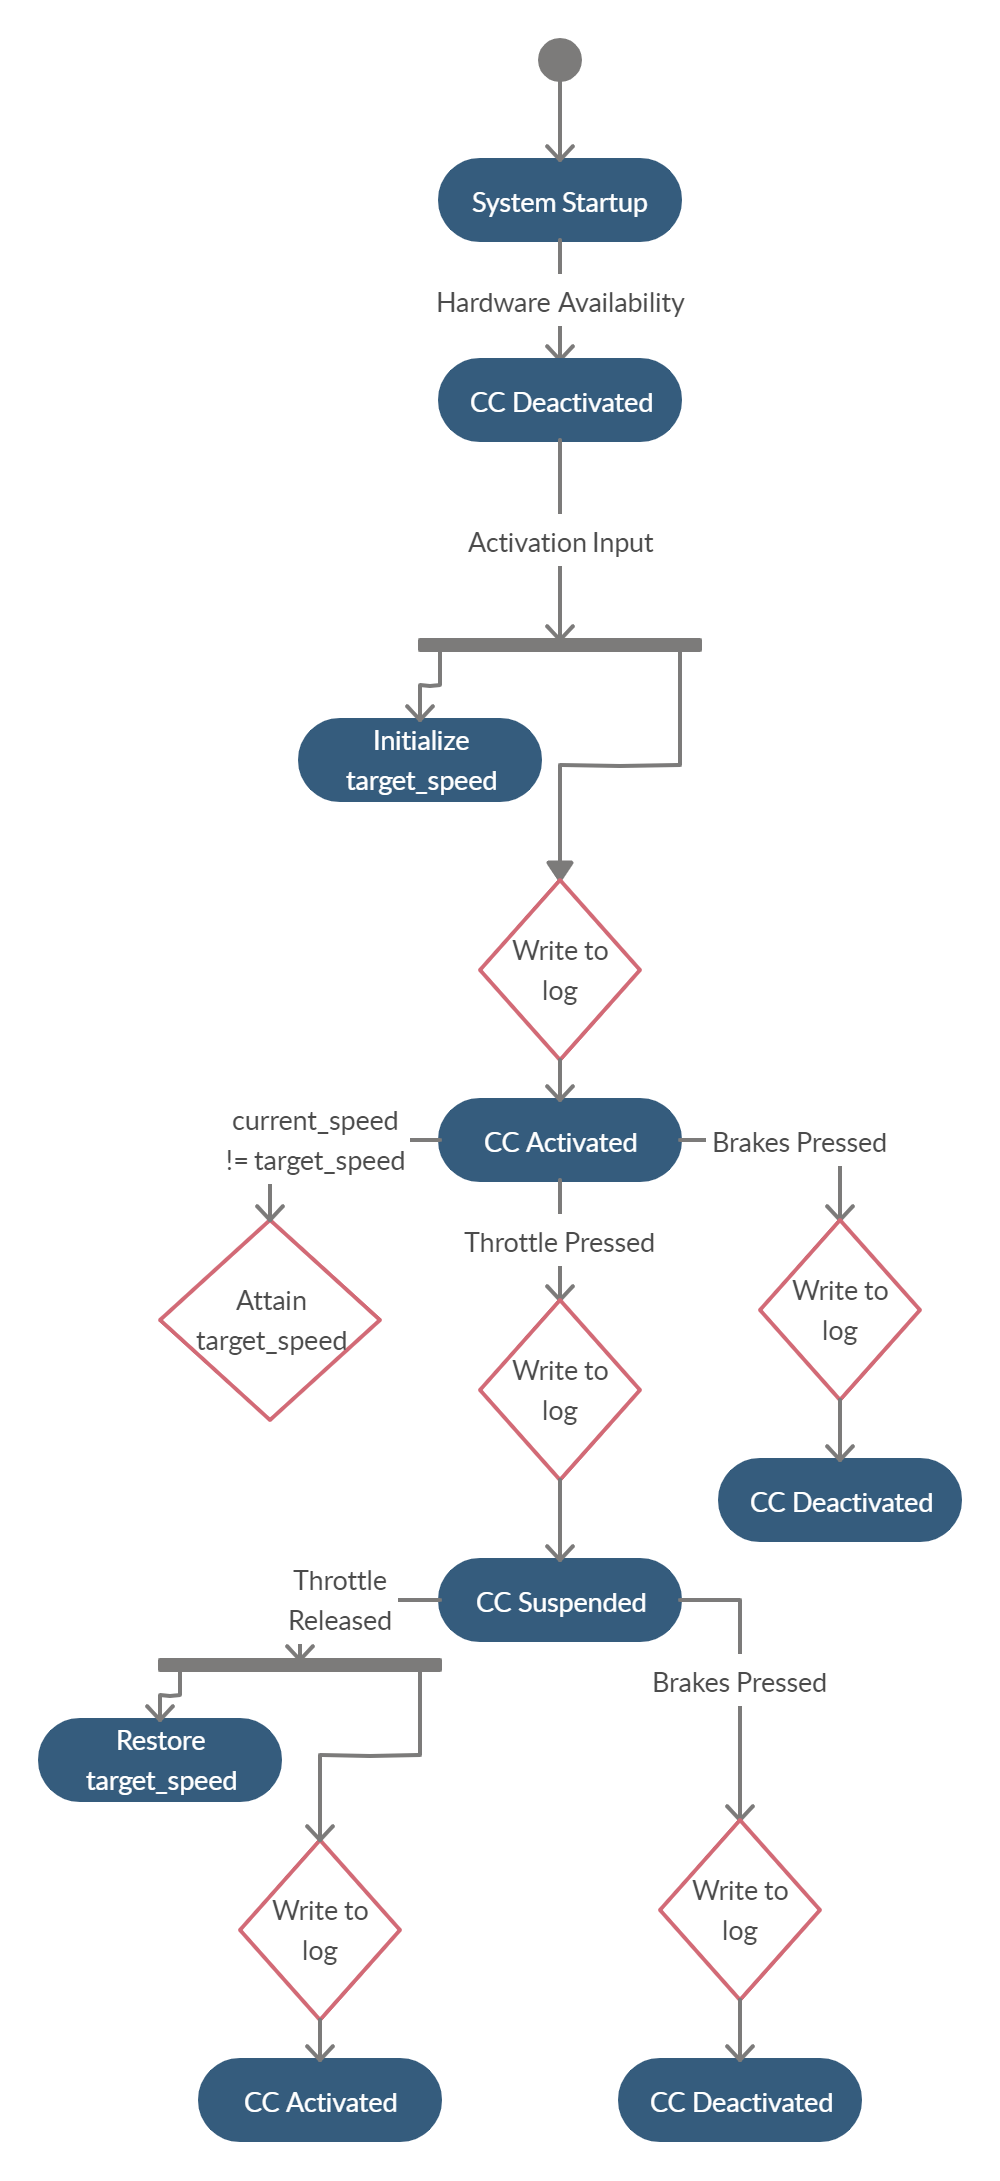
\includegraphics[scale=.26]{cs347_activity}
	\end{figure}
	
	\subsection{UML Sequence Diagram}
	\begin{figure}[!htb]
		\centering
		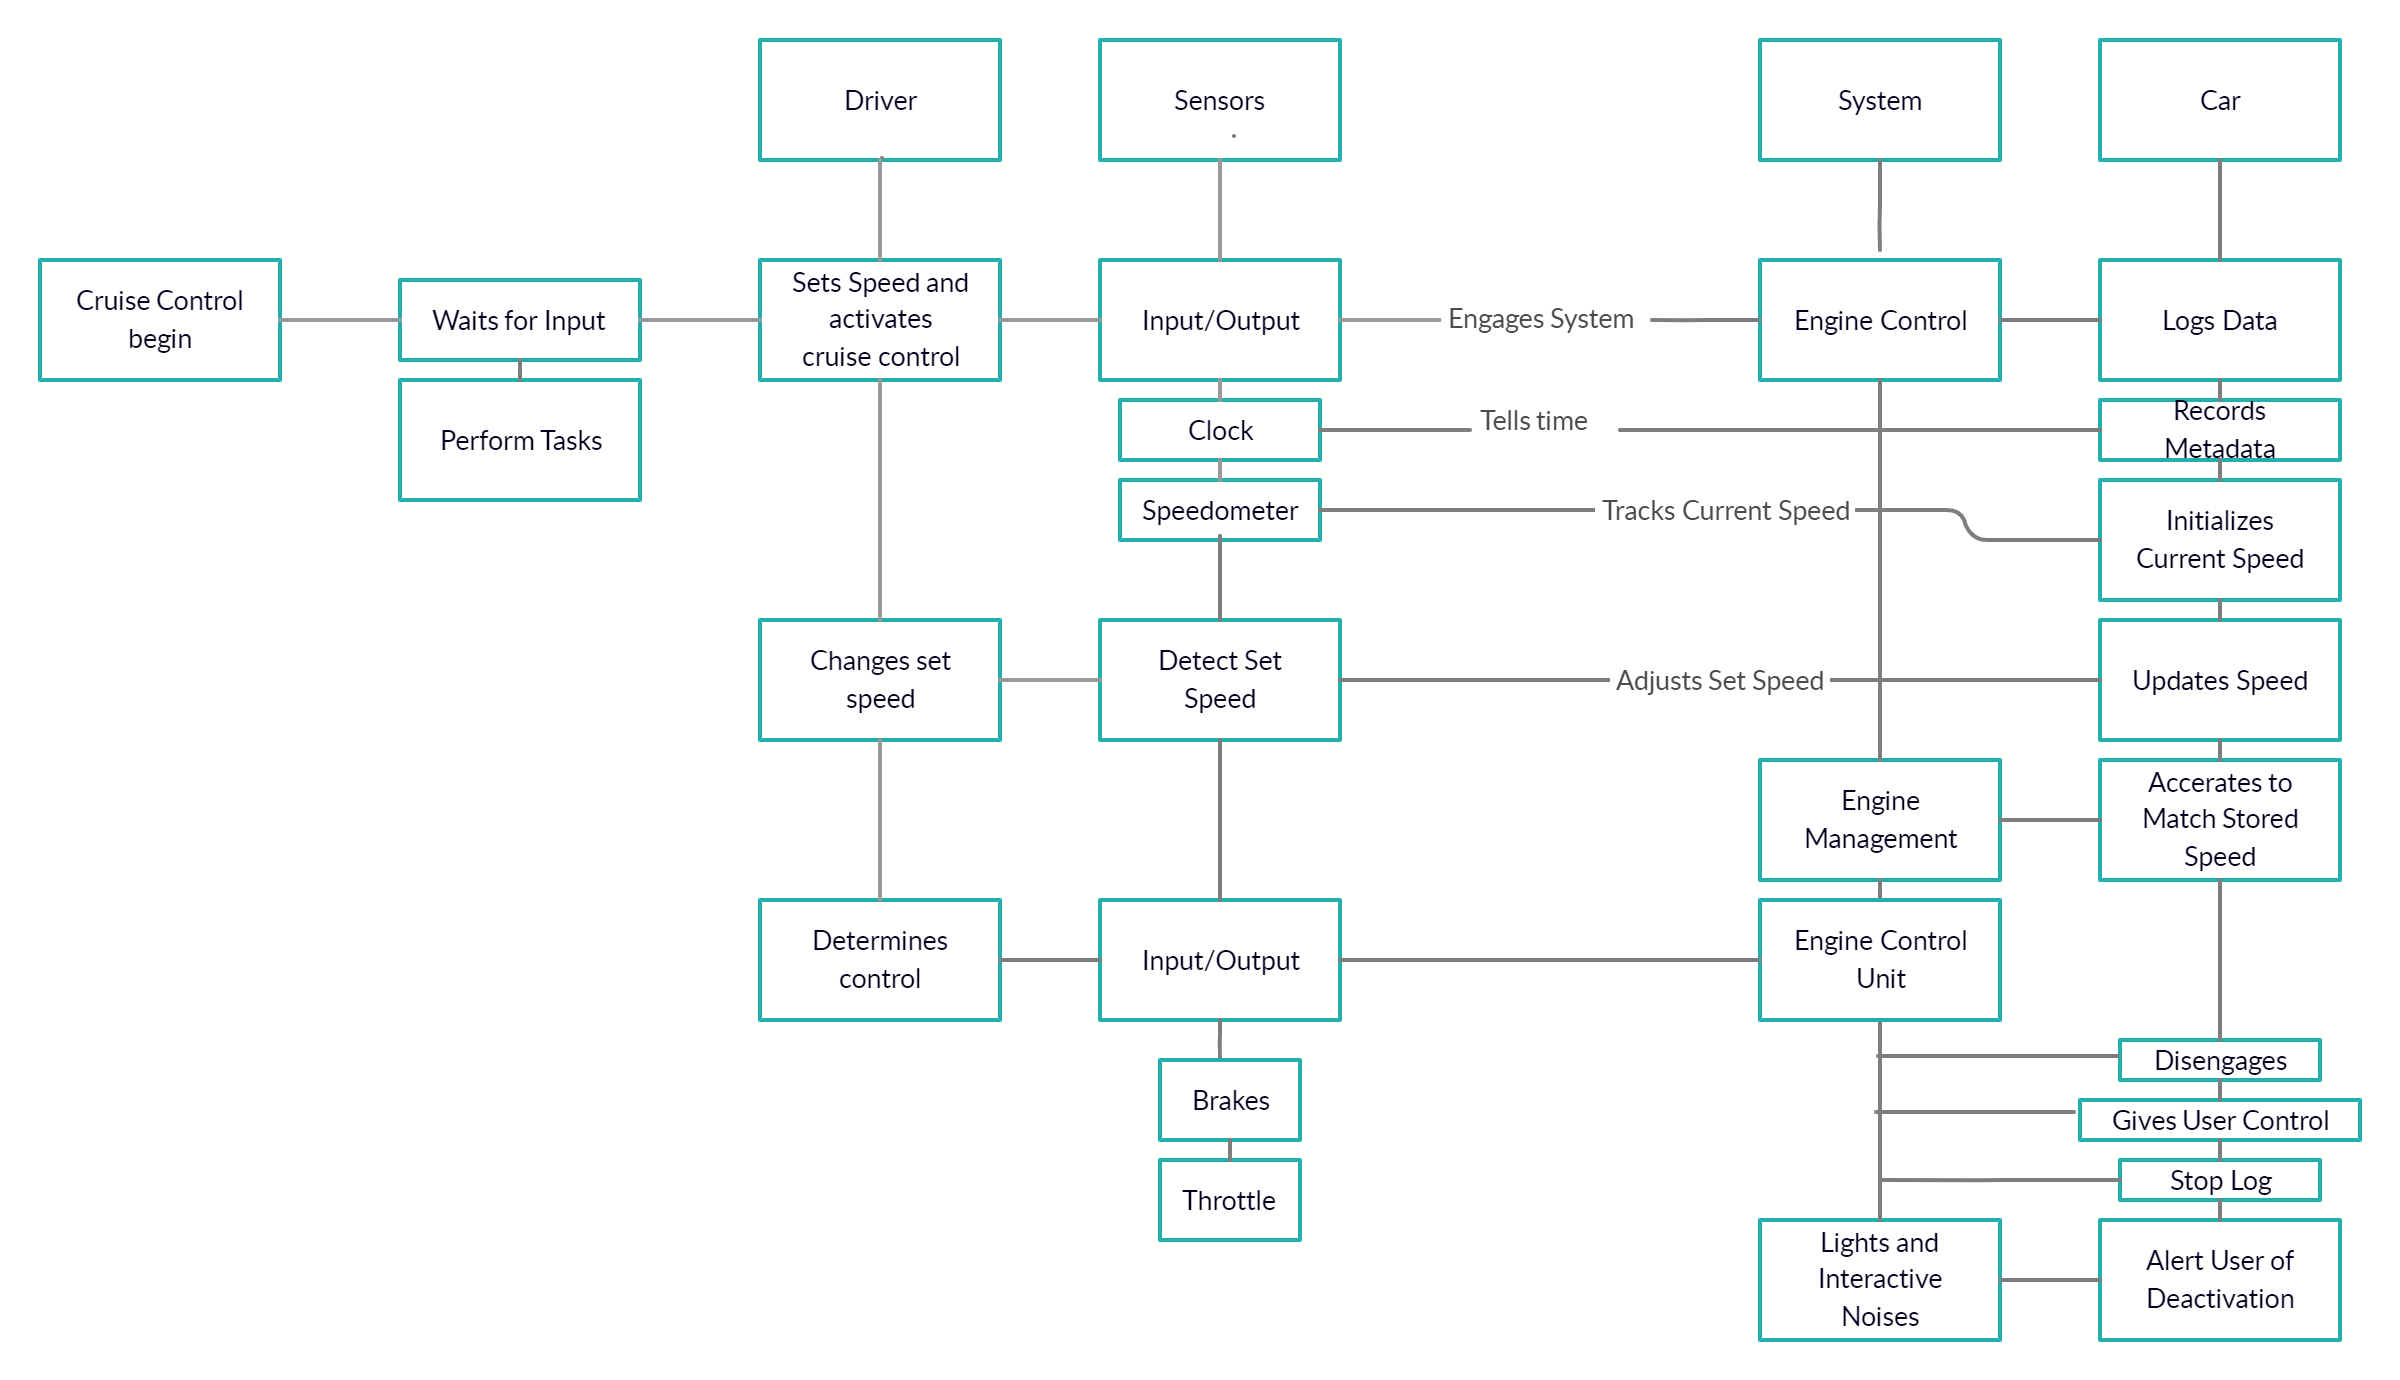
\includegraphics[scale=0.18]{cs347_sequence}
	\end{figure}
	
	\newpage
	\subsection{UML State Diagram}
	\begin{figure}[!htb]
		\centering
		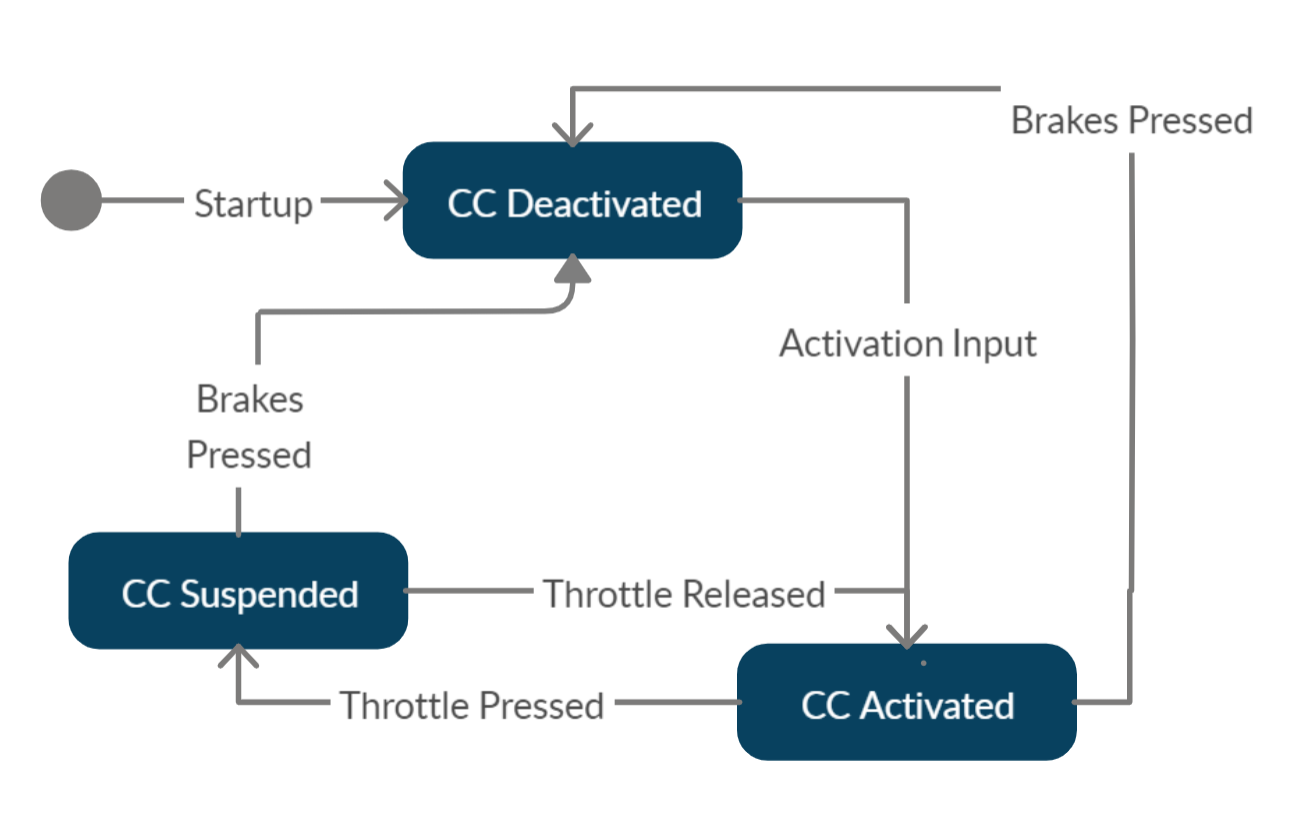
\includegraphics[scale=.55]{cs347_state}
	\end{figure}
	
	\newpage
	\section{Software Architecture}
	
	\subsection{Architecture Style}
	\indent \indent A comparison of of architecture styles we considered is as follows:
	\begin{enumerate}
		\item[5.1.1.] Data--Centered
		\begin{itemize}
			\item Pro: Facilitates communication between the backend of the software and other threaded components
			\item Con: Not designed for communication between threads
		\end{itemize}	
		
		\item[5.1.2.] Data--Flow
		\begin{itemize}
			\item Pro: Potentially many outputs allowed
			\item Pro: Facilitates parallel processing via independent branches
			\item Pro: Useful for decision--making software
			\item Con: Limited to a set sequence of operations
		\end{itemize}	
		
		\item[5.1.3.] Call Return
		\begin{itemize}
			\item Pro: Modular architecture allows easy modification
			\item Pro: Independent call trees can be run in parallel
			\item Con: Weak intercommunication
		\end{itemize}	
		
		\item[5.1.4.] Object--Oriented
		\begin{itemize}
			\item Pro: Very modular
			\item Pro: Self--documenting code
			\item Con: Limited scope forces independence of operations
		\end{itemize}	
		
		\item[5.1.5.] Layered
		\begin{itemize}
			\item Pro: Different layers are given as much access as required
			\item Pro: Highly modular; Can be changed as long as I/O remains compatible
			\item Con: Limited to communication between adjacent layers
		\end{itemize}	
		
		\item[5.1.6.] Model View Controller
		\begin{itemize}
			\item Pro: Promotes development of an interactive user interface
			\item Con: Only works as a model for user interface design
		\end{itemize}	
	\end{enumerate}
	
	\ \\ \indent Our design will follow the model view controller (MVC) architecture. The vehicle is expected to provide I/O (3.3.5--3.3.7) and will make up the model, with input being passed to the inner level of our C code that will handle system--level functions. The MVC architecture enables the system to report back to the user anything that happened within the system. The underlying system will follow a data--centered architecture, handling all I/O file descriptors in a centralized data component for ease of management.
	
	\subsection{Components, Connectors, Constraints}
	\indent\indent The components are as follows:
	\begin{enumerate}
		\item[5.2.1.] Input:
		\begin{enumerate}
			\item[5.2.1.a.] Brake sensor
			\item[5.2.1.b.] Throttle sensor
			\item[5.2.1.c.] Speedometer
			\item[5.2.1.d.] Clock
			\item[5.2.1.e.] Activation/deactivation device
			\item[5.2.1.f.] Speed adjustment device
		\end{enumerate}
		\item[5.2.2.] Output:
		\begin{enumerate}
			\item[5.2.2.a.] Activation status
			\item[5.2.2.b.] Automatic deactivation notification
			\item[5.2.2.c.] Set speed
			\item[5.2.2.d.] Failed activation
			\item[5.2.2.e.] Log file
		\end{enumerate}
	\end{enumerate}
	
	\ \\ \indent The UI will connect to the backend via function calls specified by a header file. The data required to pass through is as follows:
	\begin{enumerate}
		\item[5.2.3.] CC Deactivated
		\begin{enumerate}
			\item[5.2.3.a.] Poll activation/deactivation device for activation input
			\item[5.2.3.b.] Poll speedometer
			\item[5.2.3.c.] Write to log
		\end{enumerate}
		\item[5.2.4.] CC Activated
		\begin{enumerate}
			\item[5.2.4.a.] Poll activation/deactivation device for deactivation input
			\item[5.2.4.b.] Poll speedometer
			\item[5.2.4.c.] Poll brake sensor
			\item[5.2.4.d.] Poll throttle sensor
			\item[5.2.4.e.] Write to log
		\end{enumerate}
		\item[5.2.5.] CC Suspended
		\begin{enumerate}
			\item[5.2.5.a.] Poll brake sensor
			\item[5.2.5.b.] Poll throttle sensor
			\item[5.2.5.c.] Write to log
		\end{enumerate}
	\end{enumerate}
	
	\ \\ \indent The constraints are as follows: \\
	\indent It is possible for the user to switch between states quickly. As the log file becomes sufficiently large, it may happen that the log file is being written to while another write is requested. This case will be managed by the data store.
	
	\subsection{Control Management}
	\begin{enumerate}
		\item[5.3.1.] Control will be managed in the architecture by continuously polling for input and activation/deactivation and handing control over to the relevant components
		\item[5.3.2.] A distinct control hierarchy will not be needed for the cruise control software
		\begin{enumerate}
			\item[5.3.2.a.] The car itself already provides much of a control hierarchy
			\item[5.3.2.b.] Additionally, the cruise control is relatively simple and does not require a distinct control hierarchy
		\end{enumerate}
		\item[5.3.3.] A component ID along with any relevant data will be passed to a master control component whenever a transfer of control is desired
		\begin{enumerate}
			\item[5.3.3.a.] This master control component will perform all the necessary checks to ensure that the transfer of control is warranted, only transferring control if it is approved
		\end{enumerate}
		\item[5.3.4.] Control will be shared among components through a combination of the data store (5.4) and the master control component
		\begin{enumerate}
			\item[5.3.4.a.] The master control component will allow for shared control when necessary, e.g. running a write to the log file at the same time as speed adjustment
		\end{enumerate}
		\item[5.3.5.] The control topology will take on the shape of a star, with the master control component being the center and other components being the ``points" of the star
		\item[5.3.6.] Control will be asynchronous
	\end{enumerate}
	
	\subsection{Data Architecture}
	\begin{enumerate}
		\item[5.4.1.] Data will be accessed by components through a central data store
		\item[5.4.2.] The flow of data will be continuous and with a low latency between the sending and receiving of data
		\begin{enumerate}
			\item[5.4.2.a.] Conditions can quickly change and responding to them as soon as possible is needed to ensure that the cruise control software is not responsible for any accidents
		\end{enumerate}
		\item[5.4.3.] Data will be transferred between components via pipes
		\begin{enumerate}
			\item[5.4.3.a.] This allows for improved security by allowing components to have only a half--duplex pipe (one--way communication) for data transferal or a full--duplex pipe (two--way communication)
		\end{enumerate}
		\item[5.4.4.] Individual data components managed by the central data store will exist
		\begin{enumerate}
			\item[5.4.4.a.] Several components will need to regularly read from or write to the same data sources
			\item[5.4.4.b.] Creating separate data components for these interactions will increase the organization of the software architecture
		\end{enumerate}
		\item[5.4.5.] Functional components will use the data components to read relevant data
		\item[5.4.6.] Functional components will use the data components to write or send relevant data
		\item[5.4.7.] The data components will be active
		\begin{enumerate}
			\item[5.4.7.a.] The data components will constantly fetch data to ensure that it is up--to-date
			\item[5.4.7.b.] The use of stale data could result in unwanted behavior or even accidents due to changing conditions
		\end{enumerate}
	\end{enumerate}
	
	\subsection{Architectural Designs}
	
	\subsubsection{Architectural Context Diagram}
	\begin{figure}[!htb]
		\centering
		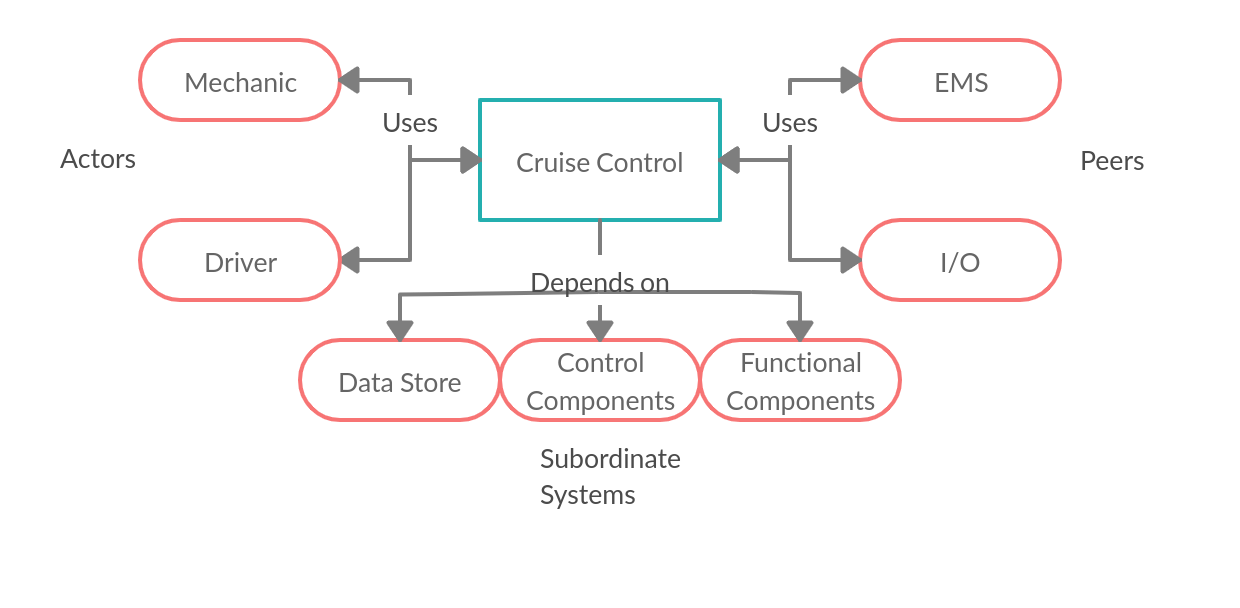
\includegraphics[scale=.34]{cs347_5a}
	\end{figure}
	
	\subsubsection{UML Relationships for Function Archetypes}
	\begin{figure}[!htb]
		\centering
		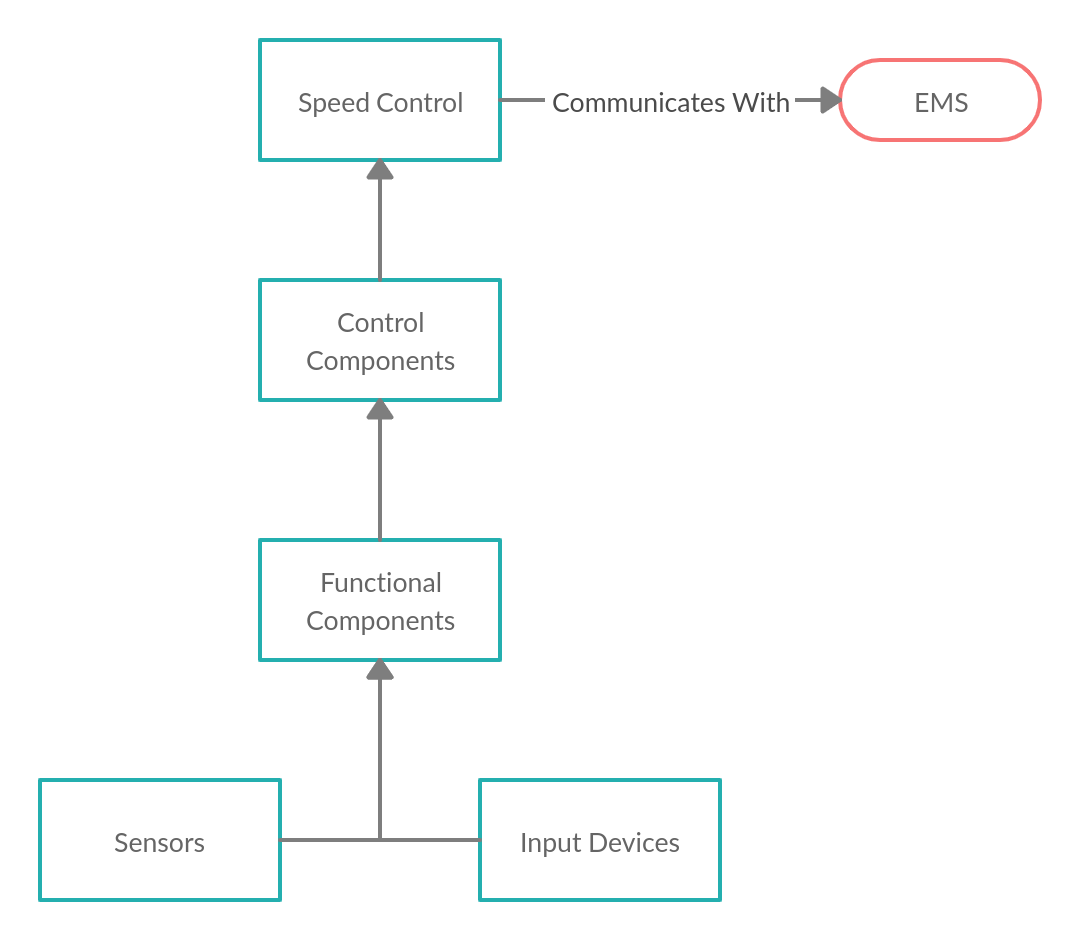
\includegraphics[scale=.28]{cs347_5c}
	\end{figure}
	
	\newpage
	\subsubsection{Architectural Structure with Top--Level Components}
	\begin{figure}[!htb]
		\centering
		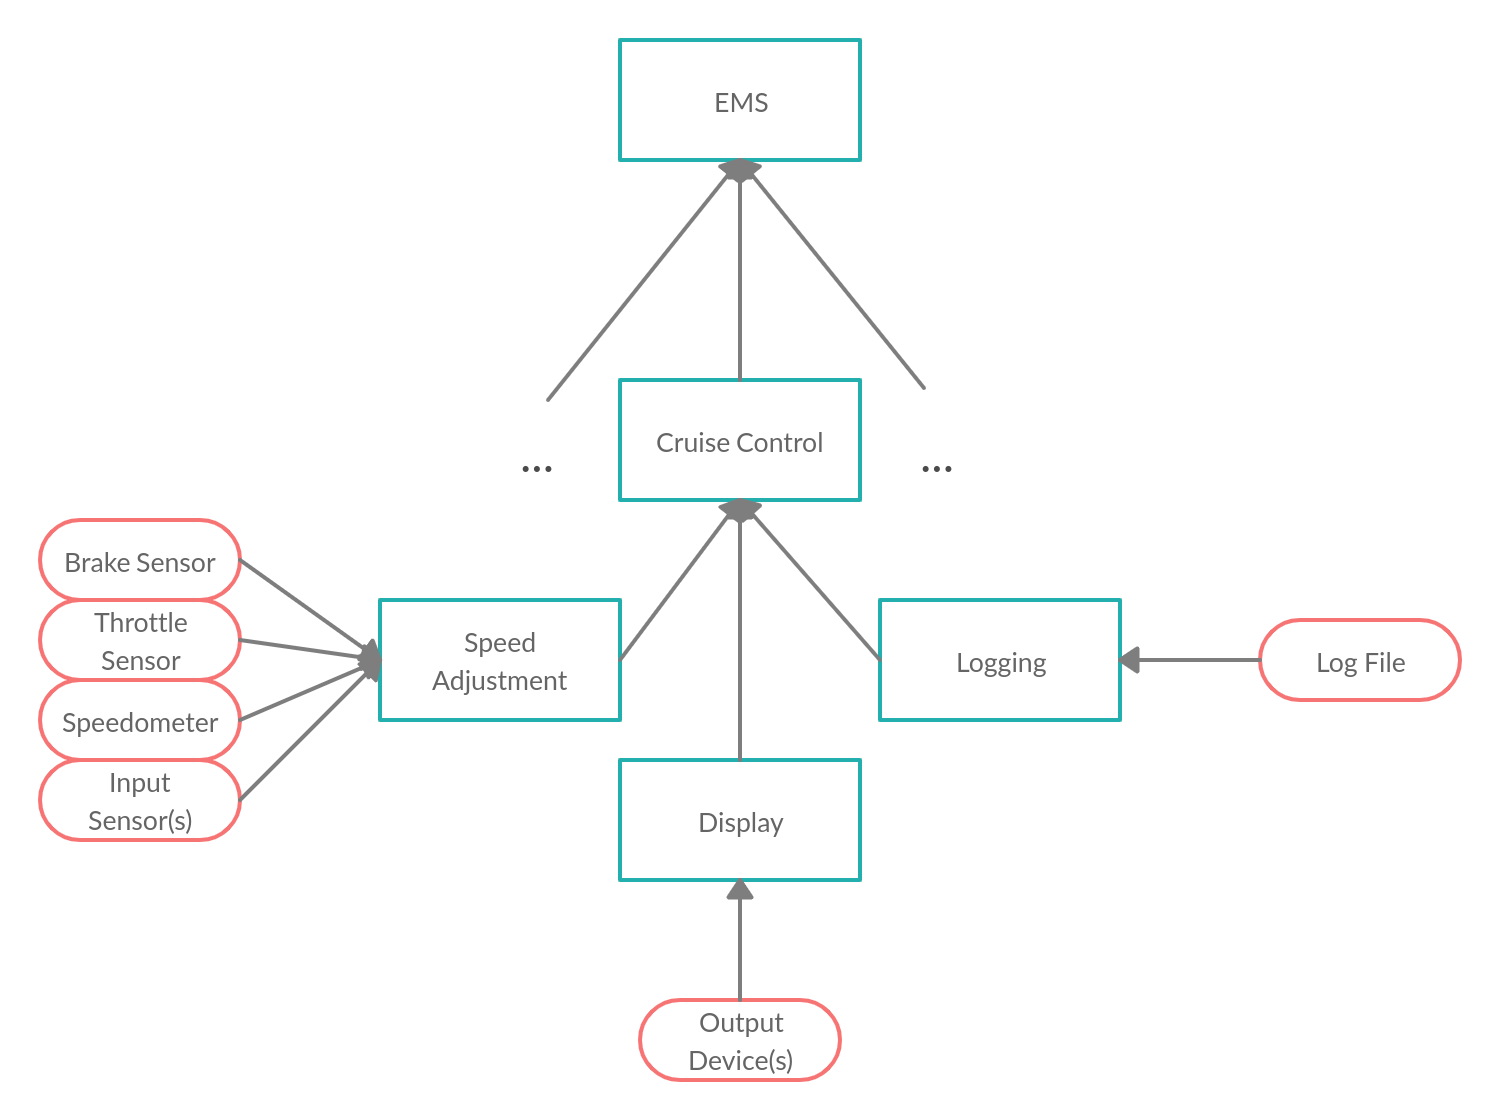
\includegraphics[scale=.28]{cs347_5b}
	\end{figure}
	
	\subsection{Issues}
	\begin{itemize}
		\item There is no known way to detect system startup completion. The software, when launched, will need to be able to figure out if all devices are active and working. During this time frame, the user may try to activate cruise control, so it is necessary to figure out a way to get the system giving feedback to the user as soon as possible. --- Dom
		\item A list of potential errors and responses must be created for problem diagnosis. The output the user may see can vary depending on the manufacturer's implementation of the display protocol. Therefore the cruise control software must provide a standard set of outputs that manufacturers can expect to hook into. --- Ryan
		\item The log must be able to handle the case wherein the storage is full. Perhaps the cruise control software will one day make it into a car that lasts forever; the log file will eventually fill up. Some method must be developed to avoid the log file from becoming ineffective. --- Michael
	\end{itemize}
	
\end{document}
